\documentclass{beamer}
\mode<presentation>
\usepackage{amsmath}
\usepackage{amssymb}
%\usepackage{advdate}
\usepackage{graphicx}
\graphicspath{{../figs/}}
\usepackage{adjustbox}
\usepackage{subcaption}
\usepackage{enumitem}
\usepackage{multicol}
\usepackage{mathtools}
\usepackage{listings}
\usepackage{url}
\def\UrlBreaks{\do\/\do-}
\usetheme{Boadilla}
\usecolortheme{lily}
\setbeamertemplate{footline}
{
  \leavevmode%
  \hbox{%
  \begin{beamercolorbox}[wd=\paperwidth,ht=2.25ex,dp=1ex,right]{author in head/foot}%
    \insertframenumber{} / \inserttotalframenumber\hspace*{2ex} 
  \end{beamercolorbox}}%
  \vskip0pt%
}
\setbeamertemplate{navigation symbols}{}
\let\solution\relax
\usepackage{gvv}
\lstset{
%language=C,
frame=single, 
breaklines=true,
columns=fullflexible
}

\numberwithin{equation}{section}



\begin{document}

\title{8.4.23}
\author{EE25BTECH11020 - Darsh Pankaj Gajare}
% \maketitle
% \newpage
% \bigskip
%\begin{document}
{\let\newpage\relax\maketitle}
%\renewcommand{\thefigure}{\theenumi}
%\renewcommand{\thetable}{\theenumi}

Question:\\
The curve described parametrically by $x = t^2 + t + 1$ and $y = t^2 - t + 1$ represents:
\begin{multicols}{2}
	\begin{enumerate}[label=(\Alph*)]
\item a pair of straight lines
\item an ellipse
\item a parabola
\item a hyperbola
\end{enumerate}
\end{multicols}


\solution
\begin{table}[H]
	\centering
	\caption{}
	\begin{tabular}{|c|c|}
\hline
\textbf{Variable} & \textbf{Value} \\
\hline
$A$ & $(0,-\frac{3}{2})$ \\
\hline
$m$ & $\frac{1}{2}$ \\
\hline
\end{tabular}
	\label{}
\end{table}


The parametric form can be written as
\begin{align}
\vec{x} &= \vec{a}t^2 + \vec{b}t + \vec{c}.
\end{align}
\begin{align}
	\vec{x}=\myvec{\vec{a}\\\vec{b}}^\top\myvec{t^2\\t}+\vec{c}
\end{align}
\begin{align}
\vec{x}=\myvec{1 & 1\\ 1 & -1}\myvec{t^2\\ t}+\vec{c}
\end{align}

\begin{align}
\myvec{t^2\\ t}=\frac{1}{2}\myvec{1 & 1\\ 1 & -1}
\brak{\vec{x}-\vec{c}}
\end{align}

\begin{align}
\text{Let } \vec{e}_1=\myvec{1\\ 0},\ \vec{e}_2=\myvec{0\\ 1},\ 
\end{align}
\begin{align}
	\vec{M}=\frac{1}{2}\myvec{1 & 1\\ 1 & -1},\ 
\vec{z}=\vec{x}-\vec{c}. 
\end{align}

\begin{align}
	\text{Then } \myvec{t^2\\ t}=\vec{M}\vec{z},\quad
	t^2=\vec{e}_1^\top \vec{M}\vec{z},\quad
	t=\vec{e}_2^\top \vec{M}\vec{z}.
\end{align}

\begin{align}
\text{Eliminate } t:\quad
	\vec{e}_1^\top \vec{M}\vec{z}
=
	\brak{\vec{e}_2^\top \vec{M}\vec{z}}^{2}.
\end{align}

\begin{align}
	\text{Define } \vec{w}=\vec{M}\vec{z}\ \Rightarrow\
\vec{e}_1^\top\vec{w}=\brak{\vec{e}_2^\top\vec{w}}^{2}.
\end{align}

\begin{align}
\text{In matrix form: }\
	\vec{z}^\top \vec{M}^\top \vec{e}_1\vec{e}_1^\top \vec{M} \vec{z}
-
	\vec{z}^\top \vec{M}^\top \vec{e}_2\vec{e}_2^\top \vec{M} \vec{z}
=0.
\end{align}

\begin{align}
	\text{Let } \vec{E}=\vec{e}_1\vec{e}_1^\top-\vec{e}_2\vec{e}_2^\top=\myvec{1&0\\ 0&-1},\
	\vec{Q}=\vec{M}^\top \vec{E} \vec{M}.
\end{align}

\begin{align}
	\vec{Q}
=
	\brak{\frac{1}{2}\myvec{1&1\\ 1&-1}}^\top
\myvec{1&0\\ 0&-1}
	\brak{\frac{1}{2}\myvec{1&1\\ 1&-1}}
=
\frac{1}{2}\myvec{0&1\\ 1&0}.
\end{align}

\begin{align}
	\vec{z}^\top \vec{Q} \vec{z}=0,\quad
\vec{z}=\myvec{x\\ y}-\myvec{1\\ 1}.
\end{align}

\begin{align}
\brak{x-1}\brak{y-1}
=
\frac{1}{2}\brak{y-x}^{2}
\ \Longleftrightarrow\
\brak{x-y}^{2}=2\brak{x+y-2}.
\end{align}

\begin{align}
\text{Thus the conic is a parabola.}
\end{align}


Since $\Delta=0$ the conic is a parabola.

\begin{figure}[H]
	\centering
	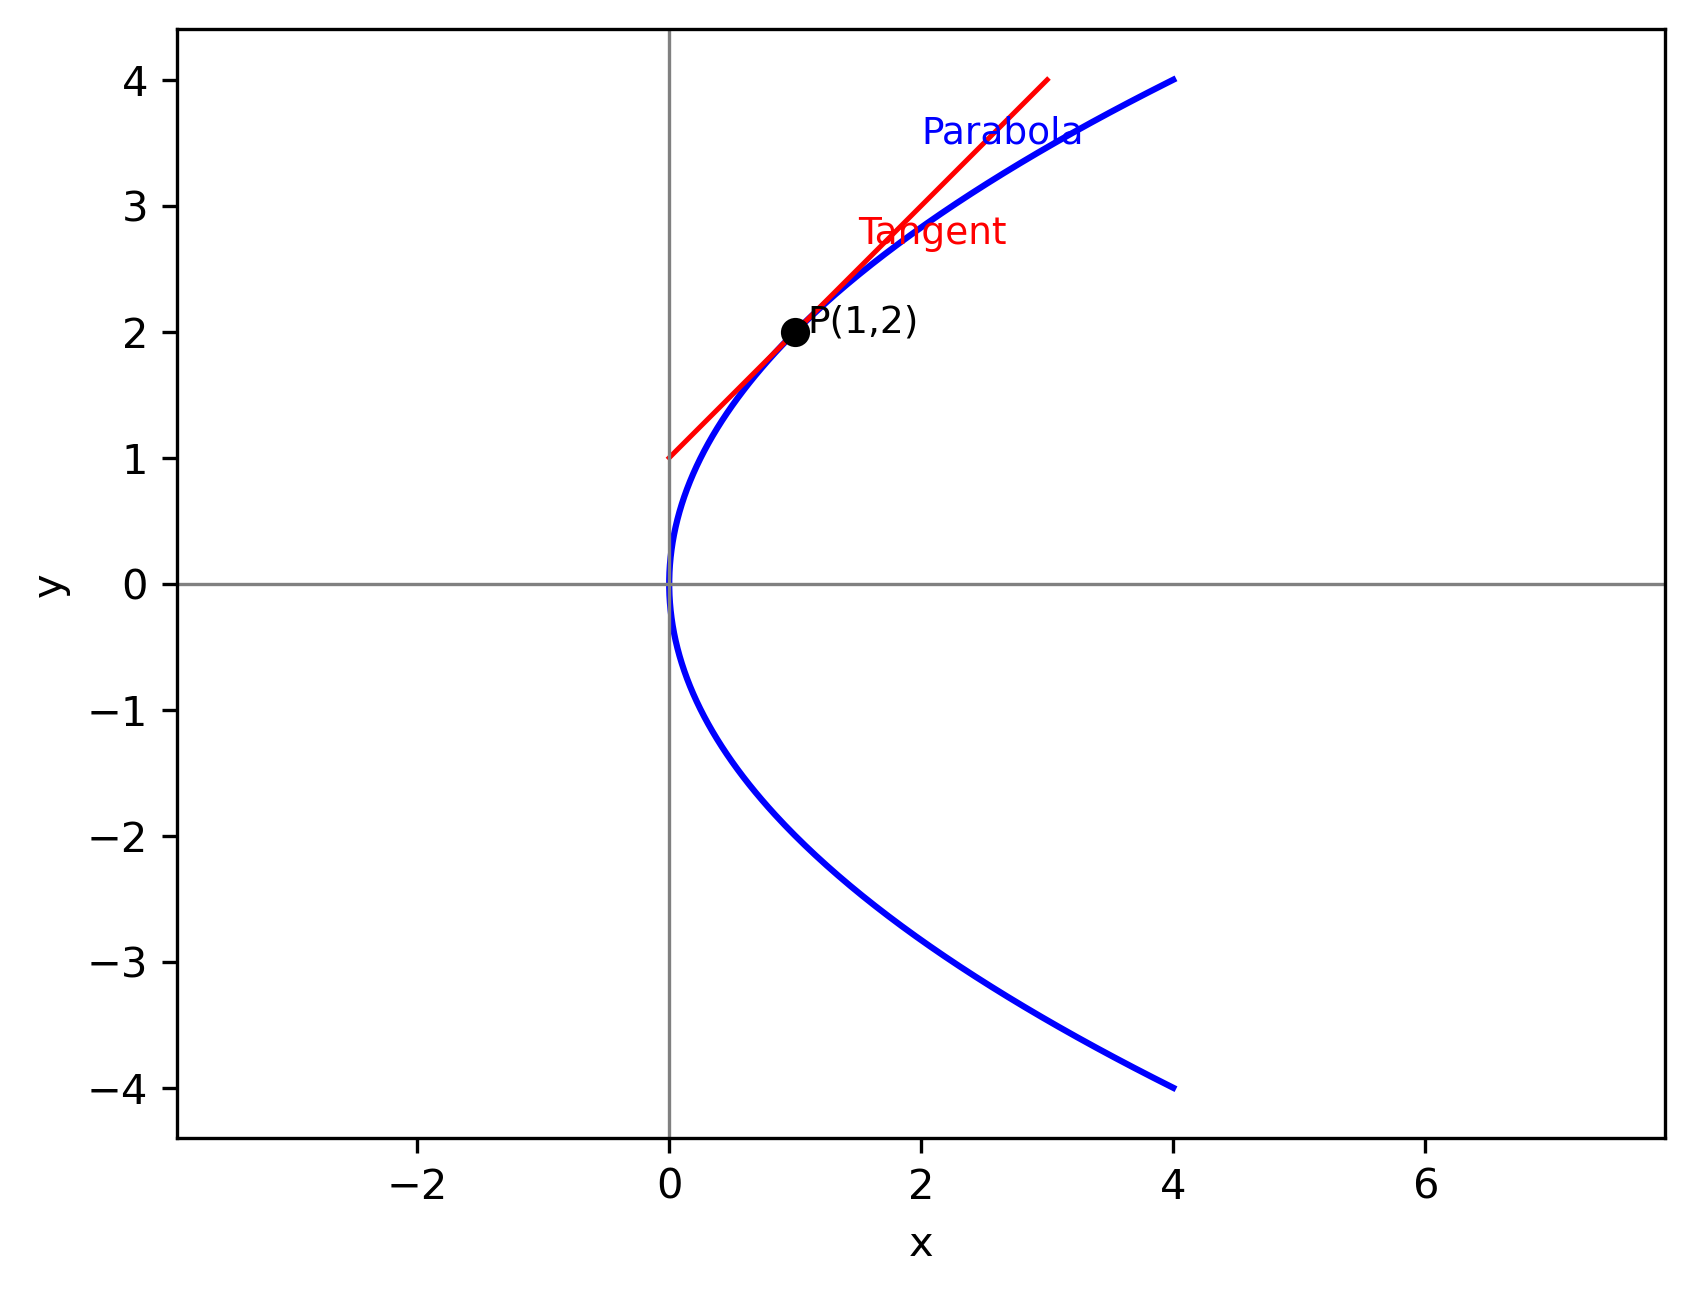
\includegraphics[scale=0.5]{img1}
	\caption*{Plot using C libraries:}
	\label{img1}
\end{figure}
\begin{figure}[H]
	\centering
	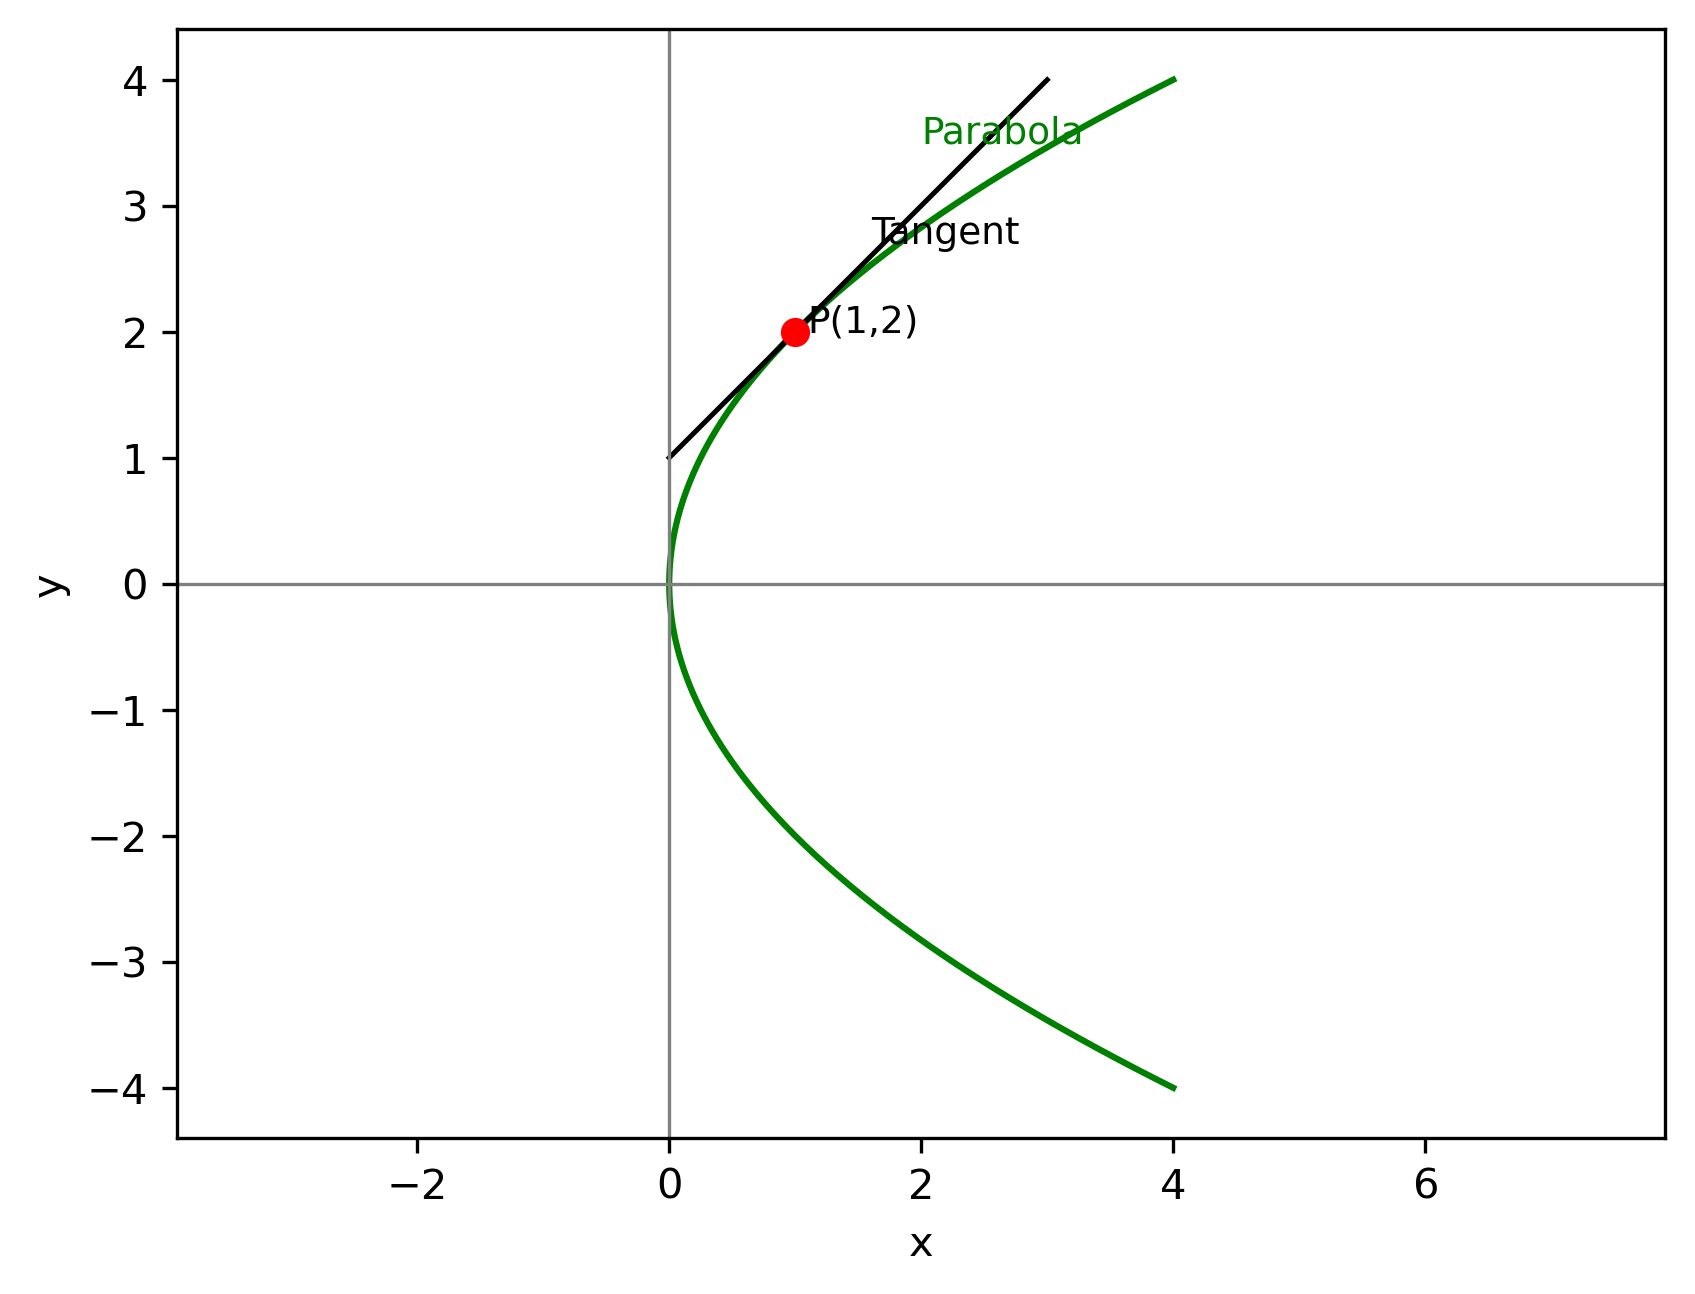
\includegraphics[scale=0.5]{img2}
	\caption*{
		Plot using Python:}
	\label{img2}
\end{figure}
\end{document}

